\documentclass[letterpaper,12pt]{exam}

\RequirePackage{comment}
\RequirePackage[hypertex]{hyperref}
\RequirePackage{GE05}
% this inputs graphicx, too
\usepackage{booktabs}

\newcommand{\NX}{\mbox{\em NX\/}}
\newcommand{\POP}{\mbox{\em POP\/}}

\def\ClassName{The Global Economy}
\def\Category{Professor David Backus}
\def\HeadName{Midterm Examination}

\printanswers 

\begin{document}
\parindent = 0.0in
\parskip = \bigskipamount
\thispagestyle{empty}%
\Head

\centerline{\large \bf \HeadName}%
%\centerline{March 9, 2005}
\centerline{Revised:  \today}

\bigskip
You have 75 minutes to complete this exam.  Please answer each
question in the space provided. You may consult one page of notes
and a calculator, but devices capable of wireless transmission are
prohibited.

I understand that the honor code applies: I will not lie, cheat,
or steal to gain an academic advantage, or tolerate those who do.

\begin{flushright}
\rule{4in}{0.5pt} \\ (Name and Signature)
\end{flushright}

%\begin{figure}[h]
%    \centering
%    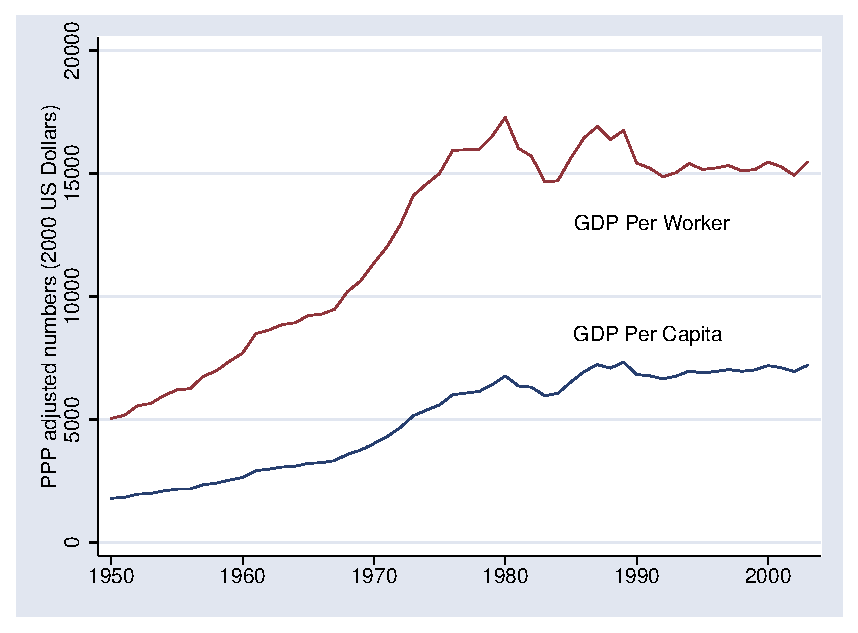
\includegraphics[scale=0.8]{pwtbramidterm07.eps}
%    \caption{GDP Per Capita and GDP Per Worker in Brazil.}
%    \label{fig:brazil}
%\end{figure}

\begin{questions}
% ======================================================================
\question {\it Growth in Korea.\/} 
Korea has been one of the world's great success stories
since the end of the Korean War, 
but there's still some debate about why.  
Was it a classic productivity story, 
or did capital formation and hours worked
play important roles?   
We know, for example, that the saving rate and hours worked 
are both relatively high.    
Your mission:  to check the numbers.  

You go to the Global Economy resource page and find:  
%
\begin{center}
\tabcolsep = 0.2in
\begin{tabular}{lrrrr}
\toprule 
Country   &  Year   &  $Y/L$   &  $K/L$ &  $K/Y$   \\
\midrule 
Korea       & 1960 &  5,964 & 9,322 & 1.52 \\
Korea       & 2007 & 47,723 & 210,432 & 4.41 \\
US          & 1960 & 37,318 & 102,655 & 2.75 \\
US          & 2007 & 84,342 & 274,080 & 3.25 \\
\bottomrule 
\end{tabular}
\end{center}
Data are from the Penn World Tables, Version 6.3.  
$Y$ is real GDP and $K$ is the stock of capital (plant and equipment, 
computed with a depreciation rate of 6\%).  
Both are PPP-adjusted and measured in 2005 US dollars.  
Employment $L$ is the number of people working.  
We refer to $Y/L$ as output per worker and 
$K/L$ as capital per worker.  

%
\begin{parts}

\part {\it Productivity.\/} 
Compute total factor productivity for each country at both dates. 
How did the ratio of Korean to US productivity change between 1960 
and 2007?  
How does it compare to the analogous ratio for output per worker?  
(10~points)

\part {\it Growth.\/}   
Compute (average annual continuously compounded) growth rates 
of output per worker for the two countries. 
Which is larger?  
(10~points)

\part {\it Growth accounting.\/}   
Decompose growth in GDP per worker into its components.  
How much of Korea's growth in output per worker was due to productivity?
How much to capital formation?  
What about the US?  
How important does Korea's high saving rate seem to be?  
(10~points)

\part {\it Hours worked.\/}   
You read in the {\it Wall Street Journal\/} 
that Koreans work exceptionally 
long hours.  
The OECD reports that the average employee in Korea worked 2266 hours in 2007,
while the average American worked only 1799 hours.  
How would this information change your calculation of TFP?
Does it change your assessment of the relative productivity 
of Korea and the US?  
(10~points)
\end{parts}

\begin{solution}
The question consists of calculations
and their interpretation (the impact of saving and hours worked
on economic performance).  
%
\begin{parts}
\part We compute productivity the usual way:  if the production
function is $ Y/L = A (K/L)^\alpha$ then $ A = (Y/L) / (K/L)^\alpha$ 
where (again as usual) $\alpha = 1/3$.  
The results are reported in the last column:  
%
\begin{center} 
\tabcolsep = 0.2in 
\begin{tabular}{lcc}
Year &  $(Y/L)_{K}/(Y/L)_{US}$  &  $A_{K}/A_{US} $  \\
\hline 
1960 & 0.16 & 0.36 \\
2007 & 0.57 & 0.62  \\
\end{tabular}
\end{center}
%
The result:  evidently there's been a much larger increase
in output per worker than in productivity.  
So it's not all productivity.  

Grading:  10 points for the calculations.  

\part Growth rates are computed using natural logarithms. 
(We denote natural logs by ``$\log$,'' 
but they're LN in Excel and on TI calculators.)   
For example, the growth rate in Korea's output per worker is 
\begin{eqnarray*}
    \gamma_{Y/L} &=&  \log (47723/5964)/47 \;\;=\;\; 0.0442 \;\;=\;\; 4.42\% .
\end{eqnarray*}
The same calculation for the US gives us a growth rate of 1.73\% per year.  
It's clear that Korea grew faster --- in fact, we knew that from 
the previous question, because the ratio of Korea to the US rose sharply.  

Grading:  10 points for the calculations.  

\part The usual growth accounting exercise.  
The numbers are  
\begin{eqnarray*}
    \mbox{General:} && \gamma_{Y/L} \;=\; \gamma_A + \alpha \gamma_{K/L} \\
    \mbox{Korea:} && 4.42  \;=\; 2.21  +  2.21   \\
    \mbox{US:} &&  1.73 \;=\; 1.04  + 0.70 .
\end{eqnarray*}
Compared to the US, Korea's growth rate of productivity is more than twice 
as large.  
But the contribution of capital per worker is three times as large.
Productivity still accounts for half of the growth in output per worker, 
but that leaves half for capital.  

You can see the same thing in several of the numbers here:  
capital per worker has been more important in Korea than in the US.
In that sense, the high saving rate has played a role.  

Grading:  8 points for the calculations, 2 for noting the connection
between the growth in capital per worker and saving.  

\part This question is intentionally more demanding, 
designed to give experts a chance to show off. 
Here we modify the production function to include hours of work:
$ Y/L = A (K/L)^\alpha h^{1-\alpha} $.
As a result, productivity (``corrected'' for hours worked)
is now 4.65 in Korea and 8.78 in the US.  
(The use of hours data changes the units.)
Relative productivity is 0.53, 
which is considerably less than the ratio of 0.62 we found earlier.
In words:  part of what we attributed to productivity before 
was really long hours.
Put another way:  Korea looks better (relative to the US) 
in a comparison of output per worker than in a comparison
of TFP, because output per worker includes a contribution 
from long hours.  
We can't assess the contribution to growth, however, 
because we're missing the 1960 hours data.  

Grading:  4 points for the formula, 4 for the calculation, 
and 2 for a sensible comment about what it means.  

\end{parts}
\end{solution}

%\pagebreak \phantom{xx} \pagebreak %\phantom{xx} \pagebreak
% ======================================================================
\question {\it Ghana v. India.\/} 
As a summer intern at Booz \& Company, you have been asked to 
prepare a short report on the possibility of 
opening call centers in Ghana aimed at the US market.  
Your report would serve as input to a sales pitch to Genpact, 
the global outsourcing firm, 
to help them identify attractive locations to expand their business.  
Like other companies in this space, Genpact started in India, 
whose low wages and large population of educated English-speakers
made it a good choice.
Now, with business growing and wages rising in India, 
Genpact is expanding into new countries.   
Ghana is a former British colony that has been growing rapidly 
in recent years after a period of unusually stable politics.  
Its official language is English.  

You put together a table of numbers using links from 
the resource page of your Global Economy course:   
%
\begin{center}
\tabcolsep = 0.1in
\begin{tabular}{lrrl}
\toprule 
Indicator   &  Ghana    &  India   &  Source  \\
\midrule 
GDP per capita (dollars) &  1,572 & 2,932 &  IMF \\
Literacy (\%)           &    58     &  61   &  CIA Factbook \\
Expected schooling (years) &  9 & 10  &  CIA Factbook \\
Absence of corruption (index) &  39 & 34 & Transparency Intl \\
Control of corruption (index) &  57 & 46 & World Bank \\
Government effectiveness (index) & 52 & 52 & World Bank \\
Rule of law (index)           & 51 & 58    & World Bank \\
Employment rigidity (index)   & 27 & 30 & Doing Business \\
%Employment rigidity (index)   & 27 & 30 & Doing Business \\
Severance costs (weeks of pay) & 178  & 56 & Doing Business \\
Quality of infrastructure (rank) & 76 & 89   & World Ec Forum \\
Quality of electricity (rank)  &  101 & 106  & World Ec Forum \\
Quality of education (rank)    &  74  & 37   & World Ec Forum \\
\bottomrule 
\end{tabular}
\end{center}
%
Indexes are on a scale of 100, ranks out of 133.  

Using these numbers  --- and your own experience and business judgment --- 
you jot down ideas organized around these questions:   
\begin{parts}
\part  What features of a country would 
make it a good choice for this business? 
(10~points)
\part Based on the evidence here, 
what are the strengths and weaknesses of Ghana relative to India 
as a location for this business?
(10~points)
\part Overall, would you favor expansion into Ghana?  
Why or why not?  
(10~points)
\end{parts}


\begin{solution}
The challenge here is to take a random collection 
of data and use it to form a coherent view of 
the quality of the local business environment 
{\it for this particular business\/}.
Good answers tied these measures to the needs of call centers, 
less good answers typically listed the measures and 
simply noted which country looked better.  
%
\begin{parts}
\part Here's a guess of the main issues 
in (roughly) declining order of importance:  
wages, English-speaking, literate and somewhat educated, 
flexible labor market, good telecommunications infrastructure, 
and general business-friendly environment.
Most of the indicators can be mapped into these categories.  

Grading:  10 points for something close to this or 
something logically coherent 
on its own terms, partial credit otherwise.  
It's essential that the answer address this specific business.  
 
\part Overall they're pretty similar. 
Wages are likely lower in Ghana, since GDP per capita is.   
English isn't the official language India, but it's a common 
second language and many Indians speak English.
In Ghana, English is the official language.  
Literacy and education are a little lower in Ghana, but there's not much difference.  
It's not clear how good the infrastructure is, but related measures 
(electricity, general infrastructure) are similar or somewhat better
in Ghana.  
The countries are similar on employment rigidity 
(Ghana is slightly less rigid), but Ghana has higher severance costs.
(It's not reported in the table, but 
severance payments here are for workers with 20+ years of employment, 
so the number may not be typical for this business.)
As for the general environment:  
rule of law, control of corruption, and effectiveness of government 
are all similar in the two countries.  

Grading:  10 points for similar discussion.  
 
\part I'd say the two countries are similar in most respects.
If you can run this business in India, you can probably run it in Ghana, 
where wages are lower.  
The one source of concern is severance costs --- we might
want to look more closely at this.  

Things I'd want to collect more information about:  
wages for the appropriate skilled people, 
political situation, how severance works, 
whether this quality of education measure is relevant to me.  

Grading:  10 points for this or other logical argument.  

\end{parts}
\end{solution}

%\pagebreak \phantom{xx} \pagebreak \phantom{xx} \pagebreak
% ======================================================================
\question {\it Miscellany.\/}
%
\begin{parts}
\part {\it Real and nominal.\/}
In 2009, nominal GDP in the US fell by 1.3\% and real GDP fell by 2.4\%.  
What do the two numbers represent?  Why are they different?  
(10~points) 

\part {\it Minimum wage.\/}
Milton Friedman once said that the minimum wage was 
blatant discrimination 
against people with low skills.  
What do you think he had in mind?  
Do you agree?  
(10~points) 

\part {\it Chinese wages.\/}
With Chinese wages rising rapidly, some observers 
have suggested that China will no longer be able to compete 
effectively with US producers.  
Do you agree?  Why or why not?  
(10~points) 
\end{parts}

\begin{solution}
\begin{parts}
\part Real GDP is (roughly) 
an index of quantities produced valued at base-year prices.
Any change reflects changes in the quantities, since
we are using the same prices at all dates.
Nominal GDP is the current value of good produced:  
the sum of current price times current quantity.
Changes thus reflect changes in both prices and quantities.  
The difference in their growth rates is therefore 
(approximately) the change in prices or inflation:  1.1\%. 

Grading:  9 points for defining the two concepts, 1 for noting
that inflation is the difference.  

\part Milton was a slippery devil, but this is basically right.  
One approach to this is based on our supply and demand diagram.
Here labor is homogeneous and some workers get higher wages than they would otherwise, while others aren't hired at all:  the minimum wage
prices them out of the market.  
Of course, labor isn't homogeneous, people have different skills. 
If you think (to keep things simple) that there's a range of skill, 
from low to high, 
who do you think will be left unemployed by a minimum wage?  
Why the low-skilled?   
If your skill level corresponds to \$5 an hour, 
and the minimum wage is \$6, then firms are unlikely to hire you.
On the other hand, if your skill level is \$10, the minimum wage 
is irrelevant.  

Grading:  10 points for a logical argument noting that the minimum
wage treats people differently depending on their skill.
6 points for an analysis based on the supply and demand diagram.  

\part The central issue here is that hiring is based on 
wages relative to productivity.
In our trade model, that's exactly what happened:  wages reflected
productivity.  
So if wages are going up, the question is why.  
If productivity is going up, too, there should be no impact on trade
and the statement is wrong.
That has to be the first-order effect:  we know China is growing rapidly
as productivity rises, and that must be reflected in wages.  

Grading:  10 points for a logical argument that relates wages
to productivity.  

\end{parts}
\end{solution}

\end{questions}

%\pagebreak \phantom{xx} %\pagebreak \phantom{xx} 

\vfill \centerline{\it \copyright \ \number\year \ NYU Stern
School of Business}

\end{document} 